\begin{frame}
\frametitle{``Traditional'' morphometrics}
Traditional morphometrics analyzes measurements of size (lengths, widths, masses, angles, ratios and areas).

Early analysis methods were often univariate, performing statistical analysis on each feature in isolation.

\vspace{0.25cm}
\begin{tiny}
Wikipedia contributors, ``Morphometrics,'' Wikipedia, The Free Encyclopedia, \url{http://en.wikipedia.org/w/index.php?title=Morphometrics&oldid=641987541} (accessed March 26, 2015).\par
\end{tiny}
\end{frame}


\begin{frame}
\frametitle{Criticism of univariate approaches}
\begin{quote}
``This unhappy result can be traced to the piecemeal tests which have hitherto been used. A bone or a tooth is a unit ; it is not a discrete assembly of independent measurements.''
\par \rightline{\tiny{\rm --- Jacob Bronowski \& W.M. Long (Nature, 1951)}}
\end{quote}
\begin{columns}[c]
\column{0.85\textwidth}
\begin{quote}
``The right statistical method must treat the set of variates as a single coherent matrix ; and this is, in fact, the technique of multivariate analysis.''
\par \rightline{\tiny{\rm --- Jacob Bronowski \& W.M. Long (Nature, 1951)}}
\end{quote}
\column{0.15\textwidth}
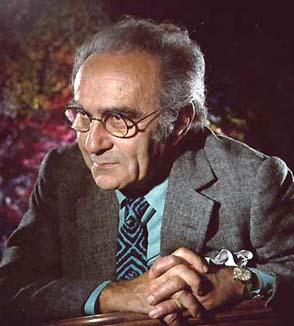
\includegraphics[width=\textwidth]{Bronowski}
\end{columns}
%\begin{tiny}
%\url{http://www.bbcshop.com/history/ascent-of-man-dvd/invt/bbcdvd1608}
%\end{tiny}
\end{frame}


\begin{frame}
\frametitle{Biological variability is multivariate}
\begin{center}
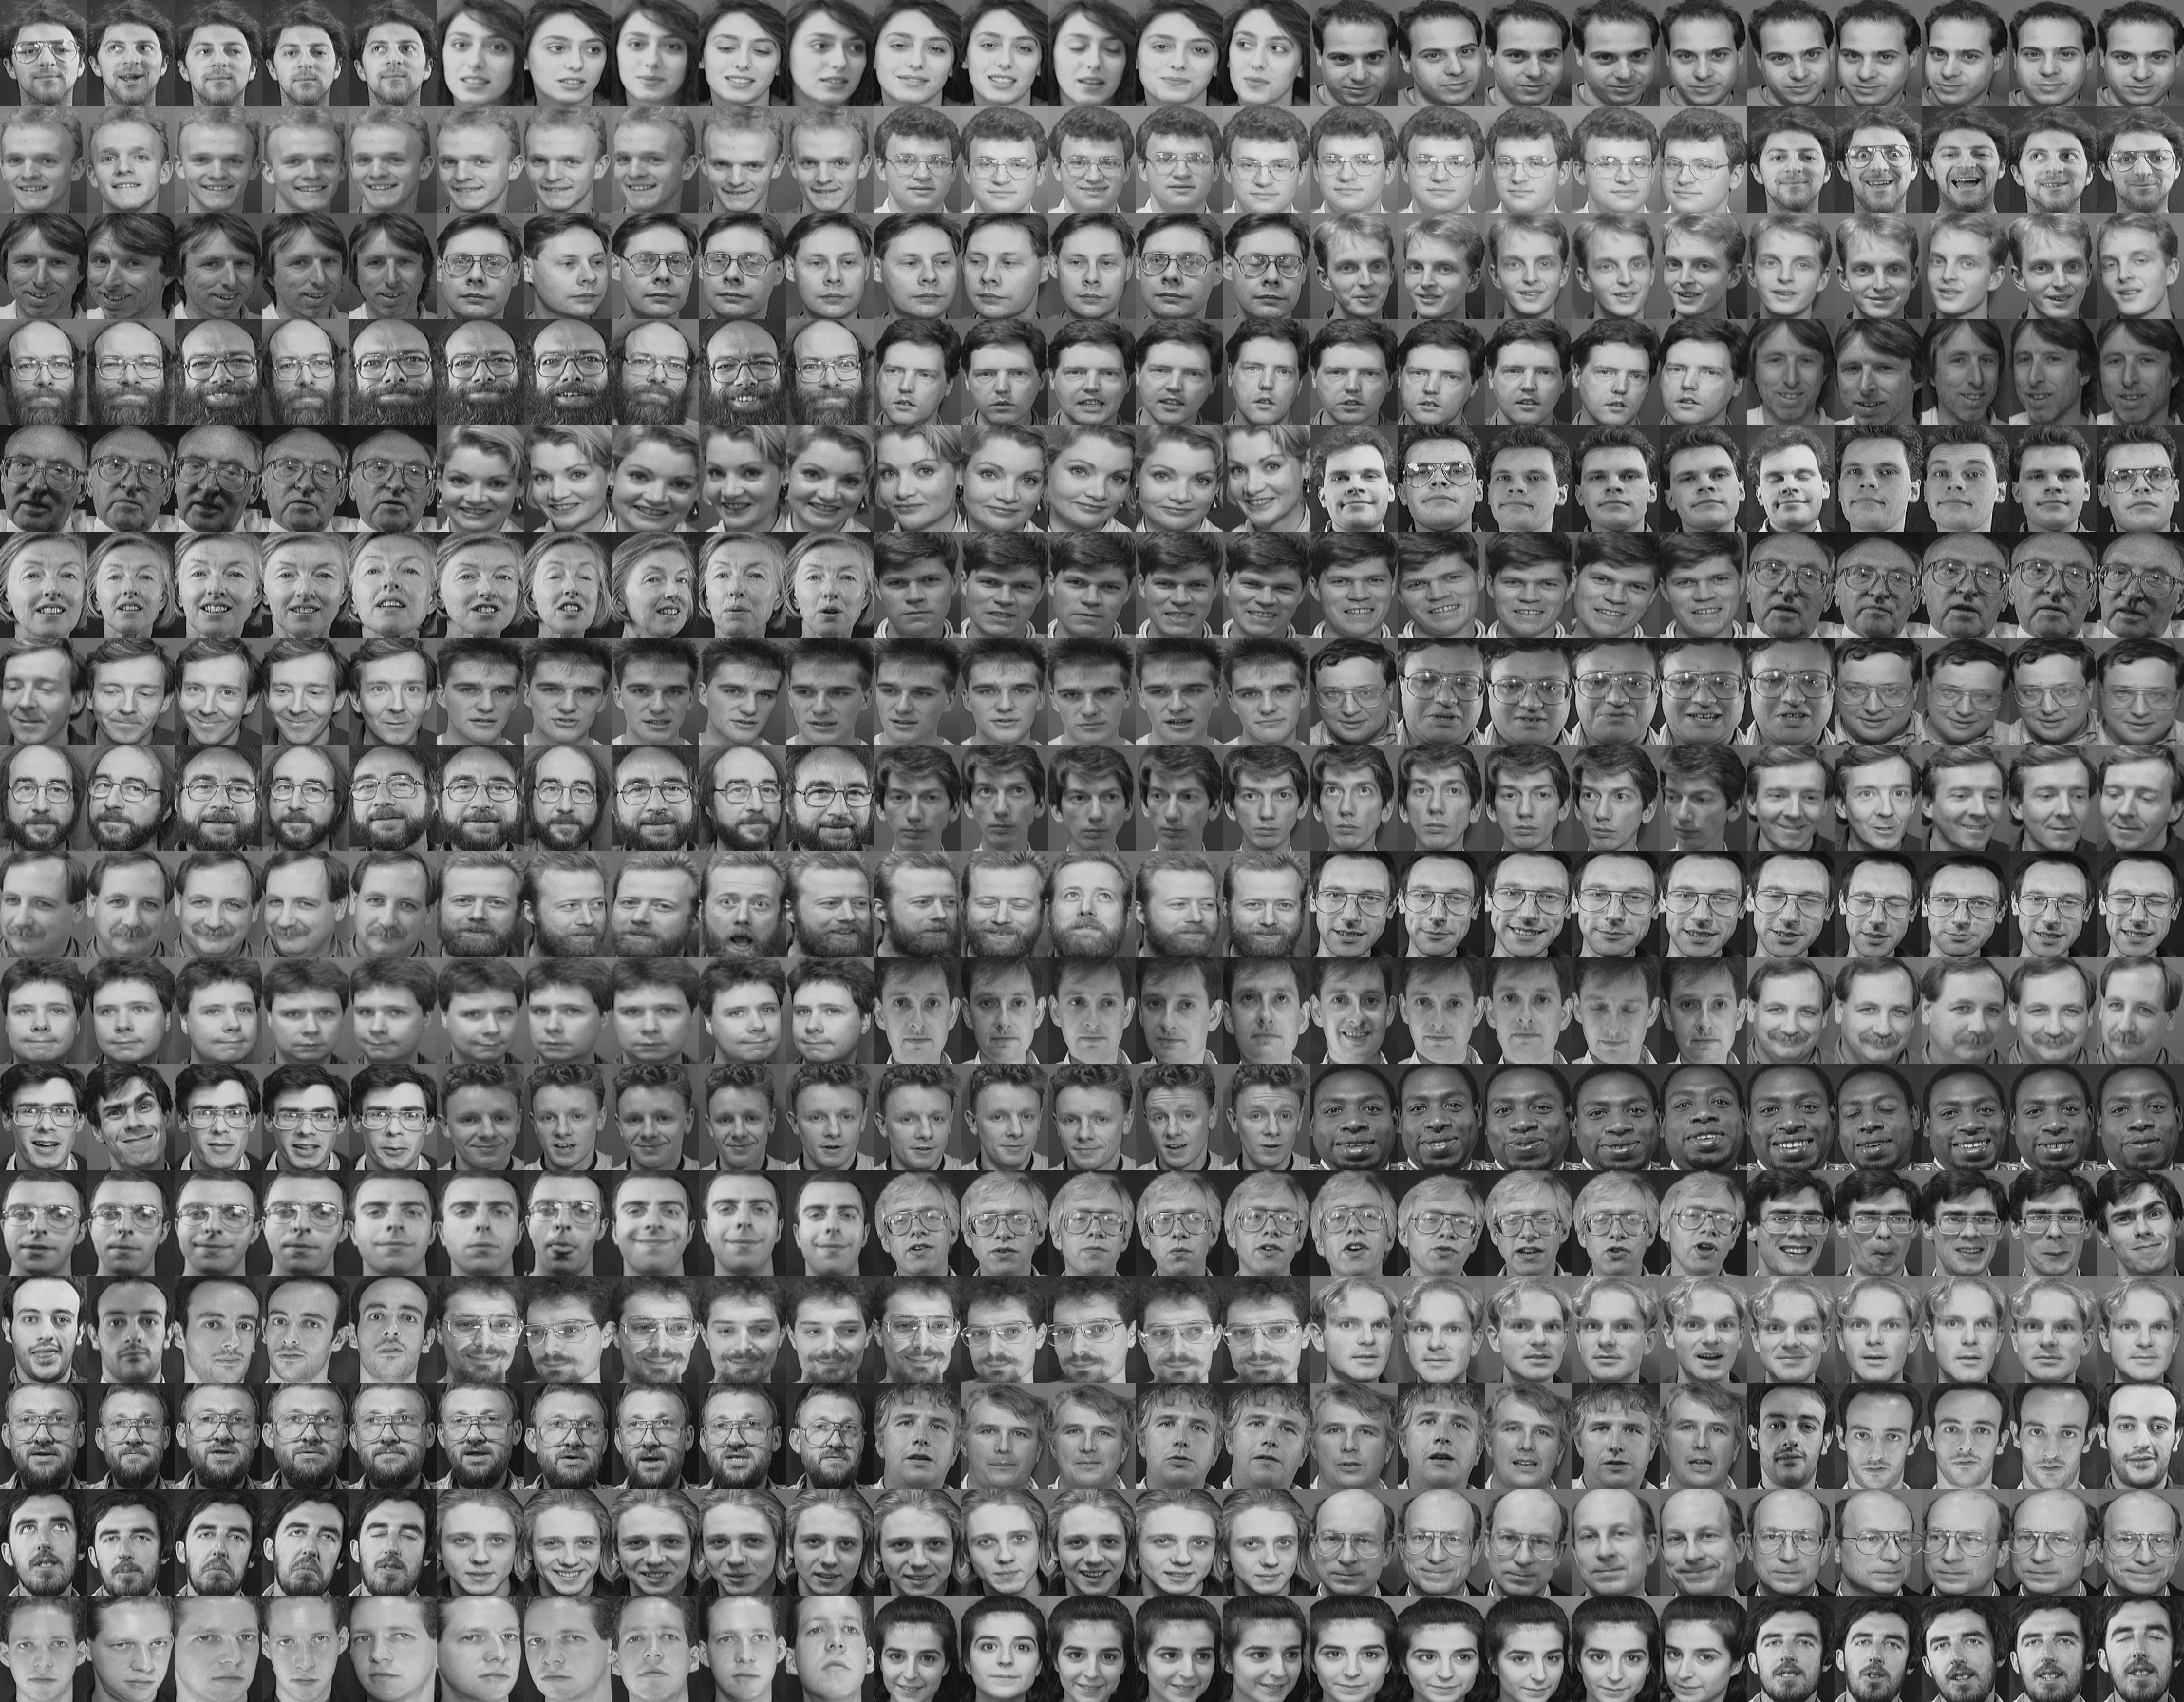
\includegraphics[height=0.6\textwidth]{faces_orig}
\end{center}
\end{frame}




